% !TeX encoding = UTF-8
% !TeX program = pdflatex
% !BIB program = biber

\documentclass[
        english,biblatex
    ]{lni}

\addbibresource{my-paper.bib}


% Standard packages
\usepackage{graphicx}
\usepackage{longtable}
\usepackage{booktabs}
\usepackage{array}
\usepackage{multirow}
\usepackage{wrapfig}
\usepackage{float}
\usepackage{colortbl}
\usepackage{pdflscape}
\usepackage{tabularx}
\usepackage{threeparttable}
\usepackage{threeparttablex}
\usepackage[normalem]{ulem}
\usepackage{makecell}

\usepackage{framed} % Needed for code blocks


% solve \tightlist error
\providecommand{\tightlist}{%
    \setlength{\itemsep}{0pt}\setlength{\parskip}{0pt}}

% solve \pandocbounded error
\providecommand{\pandocbounded}[1]{#1}



\begin{document}

% Title
        \title[]{The difference between RSE and Data Science}
    
    
    


\author[1]{Julian Dehne}{julian.dehne@gi.de}{0000-0001-9265-9619}
\author[2]{Jan Philipp Thiele}{jan-philipp.thiele@tu-braunschweig.de}{0000-0002-8901-6660}
\author[3]{Jeremy Cohen}{jeremy.cohen@imperial.ac.uk}{0000-0003-4312-2537}
\author[4]{Katrin Schöning-Stierand}{\href{mailto:katrin.schoening-stierand@uni-hamburg.de}{katrin.schoening-stierand@uni-hamburg.de}}{0000-0003-3248-8023}
\author[5]{Florian Goth}{\href{mailto:Florian.Goth@uni-wuerzburg.de}{Florian.Goth@uni-uerzburg.de}}{0000-0003-2707-4790}
\author[6]{Jan Linxweiler}{\href{mailto:j.linxweiler@tu-braunschweig.de}{j.linxweiler@tu-braunschweig.de}}{0000-0002-2755-5087}
\author[7]{Anna-Lena Lamprecht}{\href{mailto:anna-lena.lamprecht@uni-potsdam.de}{anna-lena.lamprecht@uni-potsdam.de}}{0000-0003-1953-5606}

\affil[1]{Gesellschaft für Informatik\\Bildung und Gesellschaft\\
Weydingerstraße 14-16\\10178 Berlin\\Deutschland}
\affil[2]{TU Braunschweig\\Universitätsbibliothek\\
Universitätspl. 1, 38106 Braunschweig\\Deutschland}
\affil[3]{University 3\\Department\\Address\\Country}
\affil[4]{Universität Hamburg\\Hub of Computing and Data Science\\Albert-Einstein-Ring 8\\22761 Hamburg\\Deutschland}
\affil[5]{Universität Würzburg\\Institut für theoretische Physik 1\\Am Hubland\\97070 Würzburg\\Deutschland}
\affil[6]{TU Braunschweig\\Universitätsbibliothek\\
Universitätspl. 1, 38106 Braunschweig\\Deutschland}
\affil[7]{Universität Potsdam\\Chair of Software Engineering\\An der Bahn 2\\14476 Potsdam\\Deutschland}


    \maketitle

% Abstract
        \begin{abstract}
        Die LaTeX-Klasse \texttt{lni} setzt die Layout-Vorgaben für
        Beiträge in LNI Konferenzbänden um. Dieses Dokument beschreibt
        ihre Verwendung und ist ein Beispiel für die entsprechende
        Darstellung.
    \end{abstract}
    
% Keywords
        \begin{keywords}
        LNI Guidelines \and LaTeX Vorlage
    \end{keywords}
    
% Body
    \section{What has been discussed}\label{what-has-been-discussed}

    When discussing competences for research software engineers as the
    basis of a curriculum to train Research Software engineers (RSE)
    professionals it is logical to look at the data science movement for
    inspiration. Similar to RSE, Data Science (DS) is a cross-cutting
    field that focuses on a special area within the sciences or data
    oriented businesses.

    The major computing organizations ACM and IEEE published a joint
    recommended computing curriculum which already included data
    science: the
    \href{https://www.acm.org/binaries/content/assets/education/curricula-recommendations/cc2020.pdf}{cc2020
    Computing Curriculum} already lists DS as one of the special cases
    for computing competences. Whilst DS is mentioned, research software
    engineering was absent.

    Even though it is intuitively clear that RSE is not a subclass of
    DS, there have been few attempts of differentiating the fields with
    regard to their competency sets.

    TODO insert previous research to RSE and DS: Levels of Differences
    between RSE and DS:

    \begin{itemize}
    \tightlist
    \item
      institutional
    \item
      disciplinary connections
    \item
      target groups
    \item
      political history
    \end{itemize}

    \section{RSE and DS embeddings in the Research
    Cycle}\label{rse-and-ds-embeddings-in-the-research-cycle}

    Both RSE and DS can be conceptualized as a cross-cutting concern in
    many disciplines. However, the definition and relevance of these
    issues can be generalized based on the function they fulfill in the
    research cycle Figure~\ref{fig-research_cycle}.

    \begin{figure}

    \centering{

    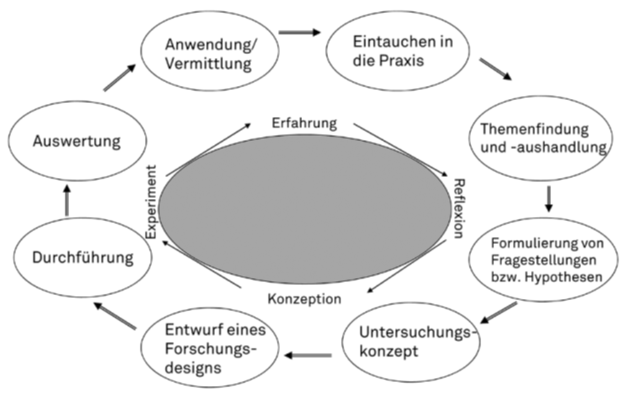
\includegraphics[width=0.7\linewidth,height=\textheight,keepaspectratio]{img/research_cycle_wildt.png}

    }

    \caption{\label{fig-research_cycle}The research cycle
    \autocite{wildt2009forschendes} integrates the typical research
    process with the learning process.}

    \end{figure}%

    There are different research processes depending on the discipline
    and the research question. However, \autocite{Dehne2021} showed that
    most of the research processes contain the following phases:

    \begin{enumerate}
    \def\labelenumi{\arabic{enumi}.}
    \tightlist
    \item
      conceptualization (developing research questions, concepts)
    \item
      design (developing the tools, instruments and concrete process
      models)
    \item
      implementation (executing the experiment, study)
    \item
      analysis \& interpretation
    \item
      dissemination (publishing, distributing, peer-review)
    \item
      reflexion and improvements
    \end{enumerate}

    For example, in the case of the field of learning technologies, the
    design phase often consists of extensive software development of
    different tools for learning. In this situation developing complex
    tools for learning can be considered as research software
    engineering. The analysis of what learners can gain from using these
    technologies can be conceived as an educational research in its own
    right. This example highlights the differences of scale in both the
    weight of the different process phases (here: phase 2) and the
    relevance of research engineering. It also shows a situation where
    research software engineering clearly differs from data science. A
    typical data science background would not enable researchers to
    build full-stack software that solves inefficiencies or
    hard-to-teach problems in education.

    In the second example a GPT-like attention model is trained to
    classify data gained from the James-Webb telescope. Due to vast
    amounts of data and the continuous stream of new data research
    software engineering is needed to implement a pipeline for data
    cleaning, data warehousing and in-time analysis. In this case, the
    analysis \& interpretation phase (4) has much more relevance.
    Another point of this is example is that data science competencies
    such as vectorization of algorithms, statistical analysis, machine
    learning etc. are interconnected with competencies from software
    engineering such as software architectures, software project
    management, and database programming. In this case the distinction
    between DS competencies and RSE competencies is very fluid.

    The main argument behind these examples is that data science and
    research software engineering have a lot in common in terms of
    software development for science but show major differences where
    they are placed in the research process. This reframes the questions
    like ``how much programming is in DS'' or ``how much engineering is
    in RSE'' to a more structured approach of which cross-cutting
    functions exist in the research cycle that require computational
    means and which functions are part of the core identity of data
    scientists or research software engineers.

    As a working hypothesis based on the example above and experience in
    the field we assume the following: {[}H1{]} RSE focuses more on
    concept development (if the research is computationally heavy),
    design, implementation and dissemination, i.e.~phases 1,2,3,6
    whereas DS focuses more on analysis, interpretation and
    dissemination (phases 4,5,6). Moreover, a second hypothesis would be
    that RSE often plays a role in shaping the context of the research
    {[}H2a{]}, such as integrating projects with similar concerns, open
    source development and institutional needs. In contrast, data
    science is exclusively embedded in the research {[}H2b{]}.

    The focal point of the following chapter will revisiting existing
    ideas for DS and RSE curricula and map the competences outlined
    there to the phases in the research process. This should give the
    abstract discussion above empirical grounding and can be used to
    test the hypothesis.

    \section{Discussion}\label{discussion}

    The lists of extracted DS and RSE competency clusters can be found
    in Appendix. We also plan to publish a full table of RSE
    competencies (and possible DS competencies) sorted by clusters. In
    terms of this top-level discussion the competency clusters are
    sufficient to compare the differences with regard to the research
    cycle.

    H1 could not be confirmed in the strict sense. Although the compiled
    competency clusters show that there is a stronger focus on certain
    stages of the research process for both RSE and DS competencies,
    both can be interpreted more generally to encompass all stages of
    the research cycle. Moreover, there are some competency description
    that seem very similar such as the focus on the research cycle for
    RSE and the data science lifecycle for DS. In terms of methodology
    simply comparing the existing mentions of competencies should not be
    regarded as the best possible proxy to the actual distribution in
    the field. A survey study asking practitioners and researchers where
    in the process they would place DS and RSE would yield far more
    convincing results. Still, self-evaluation might also be biased
    depending on the identity of the people working the in the
    respective fields.

    The most clear differences between DS and RSE are found in the
    design stage and the analysis stage. The design stage holds most of
    the competency clusters the RSE community defined. The DS
    counterpart is very general and many competencies listed there could
    in fact be construed as RSE-competencies that are imported for more
    complex cases. In contrast, the analysis stage is more connected to
    DS. This can be explained by the historic challenges software
    development faces in terms of clear-cut evaluation but also by the
    distribution of labor: if the RSE-job ends with the developed
    software and the core experiment or study uses the software as a
    tool, the analysis part is then handed over to the respective field
    specialists.

    It is very hard to both evaluate the impact of technology and also
    to evaluate the technology itself and its impact on the study.
    Comprehensive methods like Directed Acyclic Graph Modellings (DAGs)
    or Instrumental Variables try to tackle these nested evaluation
    issues but have not found widespread use.

    H2 also had to be rejected: in fact, DS seems to contain more
    aspects outside the research cycle than RSE. Even though the core
    analysis of data component is very embedded in research, DS has a
    lot of institutional, political and legal challenges. Research Data
    Management (RDM) could be named as the most prominent of these. Due
    to the strong overlap of non-research related competencies, a joint
    list competency clusters was compiled that lists the competences
    that are not research cycle related (also in the appendix).

    The long list of transversal competencies begs the question if there
    are also technical competences that overlap. Even though this was
    not the focus of the analysis, these can be easily spotted by
    investigating the shift of data analysis to artificial intelligence
    based methods. Training, fine-tuning and mainstreaming large
    language models requires more and more computing power, stable
    infrastructure and network components. On the other hand, CPU-based
    software-engineering becomes less demanding and also profits from
    AI-generated algorithm and code development. However, not all
    software engineering boils down to the current AI-hype. In summary,
    there is no clear way of generalizing whether DS or RSE need more
    and deeper understanding of computer science.

    \printbibliography

    \section{Appendix}\label{sec:appendix}

    \subsection{Glossary}\label{glossary}

    \textbf{C} A general-purpose programming language often used for
    system-level development.

    \textbf{Cpp} C++ --- an extension of C that supports object-oriented
    programming.

    \textbf{DIST} Software distribution --- the practice of packaging
    and delivering software and its dependencies.

    \textbf{DOCBB} Documentation and best practices --- ensuring code is
    understandable and maintainable.

    \textbf{DOMREP} Domain repositories --- platforms that store and
    share domain-specific research data.

    \textbf{HPC} High-Performance Computing --- using supercomputers and
    parallel processing for complex tasks.

    \textbf{MOD} Modularity --- the design principle of separating
    software into interchangeable, functional components.

    \textbf{NEW} Novel research --- work that contributes original
    insights to a scientific domain.

    \textbf{PM} Project Management --- planning, executing, and
    overseeing projects effectively.

    \textbf{Python} A high-level programming language widely used in
    data science and scripting.

    \textbf{R} A programming language and environment for statistical
    computing and graphics.

    \textbf{RSE} Research Software Engineer --- someone who applies
    software engineering skills to scientific research.

    \textbf{SP} Software publication --- the process of preparing and
    disseminating software artifacts.

    \textbf{SRU} Software reuse --- the practice of using existing
    software components in new projects.

    \textbf{STEM} Science, Technology, Engineering, and Mathematics.

    \textbf{SWREPOS} Software repositories --- systems for storing and
    managing software code and versions.

    \textbf{TEAM} Teamwork --- the ability to collaborate effectively in
    a group setting.

    \textbf{TEACH} Teaching --- the skill of communicating knowledge and
    helping others learn.

    \textbf{USERS} End users --- the scientists or researchers who rely
    on software tools.

    \subsection{DS and RSE Competences in relation to the Research
    Cycle}\label{ds-and-rse-competences-in-relation-to-the-research-cycle}

    In the following the contents of \autocite{GI2021DataScience} and
    \autocite{petersen_2025_15025246} are parsed as the most current
    examples of data science curricula in the German research context.
    The contents are inspected for obvious links to the research process
    and interpreted if no explicit connections are made.

    For the RSE side the contents of \autocite{Goth2024RSE} are used as
    a basis as well as the current state of the
    \href{https://github.com/juliandehne/RSE-Masters/blob/main/curriculum.md}{RSE-Curriculums
    project}. For the RSE competencies the RSE community has developed
    short codes. These are attached in the glossary in the appendix.

    In terms of methodology it should be noted that this approach
    follows a community-driven consensus building. It should not be
    mistaken for a review study with measurable intersubjectivity based
    on instruments like \href{https://www.prisma-statement.org}{PRISMA}.

    \emph{1. Conceptualization}

    \textbf{RSE Competencies:}

    \begin{itemize}
    \tightlist
    \item
      Understanding the research cycle (\texttt{RC})
    \item
      Conducting and leading research (\texttt{NEW})
    \end{itemize}

    \textbf{Data Science Competencies:}

    \begin{itemize}
    \tightlist
    \item
      Understanding the Data Science Lifecycle and methods selection
    \item
      Awareness of data context, purpose, and interdisciplinary
      implications (ethics, economics, legal)
    \end{itemize}

    \emph{2. Design}

    \textbf{RSE Competencies:}

    \begin{itemize}
    \tightlist
    \item
      Software Design
    \item
      Software re-use strategies (\texttt{SRU})
    \item
      Creating documented code building blocks (\texttt{DOCBB})
    \item
      Software behavior analysis (\texttt{MOD})
    \item
      Building distributable software (\texttt{DIST})
    \item
      Tool and environment configuration (\texttt{SWLC},
      \texttt{SWREPOS})
    \item
      Full-Stack Programming
    \end{itemize}

    \textbf{Data Science Competencies:}

    \begin{itemize}
    \tightlist
    \item
      Data integration \& feature engineering (ETL, pipelines, quality
      checks)
    \item
      Design of data workflows and modeling processes
    \item
      Visualization theory and editorial thinking (exploratory analysis)
    \item
      Algorithm selection and objective function definition (ML core)
    \item
      Designing responsible data usage frameworks (ethics, privacy)
    \item
      Data-oriented Programming (R, Python, Matlab etc.)
    \end{itemize}

    \emph{3. Implementation}

    \textbf{RSE Competencies:}

    \begin{itemize}
    \tightlist
    \item
      Source control, testing, CI/CD (\texttt{SWREPOS}, \texttt{DIST},
      \texttt{DOCBB})
    \item
      Working in interdisciplinary teams (\texttt{TEAM})
    \item
      Project and task management (\texttt{PM})
    \end{itemize}

    \textbf{Data Science Competencies:}

    \begin{itemize}
    \tightlist
    \item
      Deployment of data pipelines and operational models
    \item
      Tool usage (Python, R, Julia, ML libraries like scikit-learn,
      Dask)
    \item
      Executing experiments using machine learning, deep learning
    \item
      Applying project management and interdisciplinary communication
    \end{itemize}

    \emph{4. Analysis \& Interpretation}

    \textbf{RSE Competencies:}

    \begin{itemize}
    \tightlist
    \item
      Software behavior interpretation (\texttt{MOD})
    \item
      Documentation of research results and workflows
    \end{itemize}

    \textbf{Data Science Competencies:}

    \begin{itemize}
    \tightlist
    \item
      Explorative Data Analysis (EDA), multivariate visualizations
    \item
      Deep understanding of model inference and optimization strategies
    \item
      Time series analysis, pattern mining, and argumentation (Data
      Mining)
    \item
      Ethical analysis of bias, fairness, and model accountability
    \end{itemize}

    \emph{5. Dissemination}

    \textbf{RSE Competencies:}

    \begin{itemize}
    \tightlist
    \item
      Software publication and citation (\texttt{SP})
    \item
      Use of domain repositories (\texttt{DOMREP})
    \item
      Teaching and communication (\texttt{TEACH}, \texttt{USERS})
    \end{itemize}

    \textbf{Data Science Competencies:}

    \begin{itemize}
    \tightlist
    \item
      Reporting results and dashboards
    \item
      FAIR principles and reproducibility practices
    \item
      Preparation of software and models for open science platforms
    \item
      Communicating findings across disciplinary and public boundaries
    \end{itemize}

    \emph{6. Reflexion and Improvements}

    \textbf{RSE Competencies:}

    \begin{itemize}
    \tightlist
    \item
      Continuous integration and testing (\texttt{SWLC}, \texttt{MOD})
    \item
      Feedback-informed iterative development
    \item
      Mentoring, community involvement, and ethics (\texttt{TEAM},
      \texttt{USERS})
    \end{itemize}

    \textbf{Data Science Competencies:}

    \begin{itemize}
    \tightlist
    \item
      Critical reflection on model performance and bias
    \item
      Model tuning, reengineering, and lifecycle updates
    \item
      Reinforcement learning and emerging AI models
    \item
      Responsible innovation, economic awareness, data sovereignty
    \item
      Application of Data Science in real-world domain projects
    \end{itemize}

    \subsection{DS and RSE competencies outside the Research
    Cycle}\label{ds-and-rse-competencies-outside-the-research-cycle}

    This section collects transversal competencies in Data Science and
    Research Software Engineering (RSE) that support research but are
    not tied to a specific phase of the research process.

    \emph{1. Ethical and Legal Awareness}

    \textbf{Data Ethics}

    \begin{itemize}
    \tightlist
    \item
      Awareness of bias and fairness in data
    \item
      Model transparency, explainability, and accountability
    \item
      Risk and impact assessment (e.g., algorithmic decision-making)
    \item
      Ethical reflection throughout the data lifecycle
    \end{itemize}

    \textbf{Data Privacy and Legal Contexts}

    \begin{itemize}
    \tightlist
    \item
      National and international data protection laws
    \item
      Differentiation between personal and non-personal data
    \item
      Licensing and data usage regulations
    \item
      Data compliance skills
    \end{itemize}

    \emph{2. Interdisciplinary Collaboration}

    \textbf{Communication and Project Skills}

    \begin{itemize}
    \tightlist
    \item
      Project planning and evaluation
    \item
      Communication across disciplines and with non-experts
    \item
      Knowledge of marketing and dissemination strategies
    \end{itemize}

    \textbf{Domain Integration and Labs}

    \begin{itemize}
    \tightlist
    \item
      Ability to adapt and apply methods in various domains
    \item
      Independent and team-based domain project execution
    \item
      Research data management within domains
    \item
      Interdisciplinary labs as agile learning environments
    \end{itemize}

    \emph{3. Computer Science Specialties}

    \textbf{Various CS specializations such as}

    \begin{itemize}
    \tightlist
    \item
      database programming
    \item
      constraint programming
    \item
      machine learning
    \item
      algorithmic design
    \item
      \ldots{}
    \end{itemize}

% Bibliography



\end{document}
